\chapter{Impacto Ambiental de los Materiales Poliméricos}
\label{cap:ambiental}

El éxito socioeconómico indiscutible de los plásticos de un solo uso durante las últimas décadas ha dado lugar a una crisis de residuos e impacto ecológico global. Su persistencia física en el medio ambiente y su baja degradabilidad natural plantean serios desafíos ecológicos.

\section{Persistencia de Plásticos Sintéticos y Microplásticos}

Los polímeros petroquímicos tradicionales como el polietileno (PE) y el polipropileno (PP) poseen una cadena principal compuesta exclusivamente por enlaces covalentes simples carbono-carbono y carbono-hidrógeno extremadamente estables. Esta estructura apolar e inerte carece de grupos funcionales sensibles a la hidrólisis química o al ataque enzimático de microorganismos en la biosfera. Por ende, su degradación natural en vertederos requiere de varios siglos.

Bajo la radiación ultravioleta (UV) solar directa y la erosión física mecánica en ecosistemas marinos, los plásticos macroscópicos se fragmentan abióticamente en partículas diminutas menores a 5 milímetros denominadas microplásticos primarios y secundarios, capaces de bioacumularse a través de las redes tróficas marinas.

\section{Polímeros Biodegradables y de Fuentes Renovables}

Para mitigar esta problemática, se investigan los bioplásticos, clasificándolos formalmente bajo dos ejes distintos:

\begin{description}
    \item[Bio-basados:] Polímeros procedentes de fuentes agrícolas renovables en lugar de combustibles fósiles petroquímicos (e.g., bio-polietileno sintético, que conserva exactamente la misma no-biodegradabilidad que su contraparte fósil).
    \item[Biodegradables:] Polímeros capaces de descomponerse biológicamente por acción de microorganismos (bacterias, hongos) bajo condiciones específicas en dióxido de carbono, agua y biomasa. Ejemplos líderes son el Poli(ácido láctico) (PLA) obtenido de la fermentación del almidón de maíz, y los Polihidroxialcanoatos (PHAs) sintetizados intracelularmente por bacterias.
\end{description}

\begin{figure}[h]
    \centering
    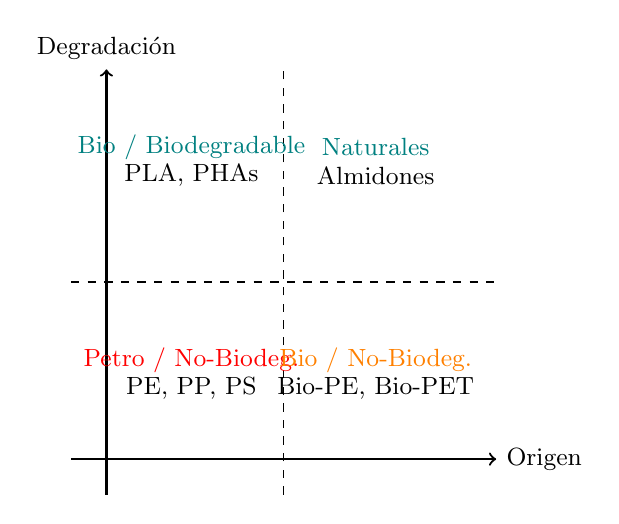
\begin{tikzpicture}[scale=0.9]
        \draw[thick, ->] (-0.5,0) -- (5.5,0) node[right] {\small Origen};
        \draw[thick, ->] (0,-0.5) -- (0,5.5) node[above] {\small Degradación};
        
        \draw[dashed] (2.5,-0.5) -- (2.5,5.5);
        \draw[dashed] (-0.5,2.5) -- (5.5,2.5);
        
        % Etiquetas de cuadrantes
        \node at (1.2,4) {\small PLA, PHAs};
        \node at (1.2,4.4) [color=teal] {\small Bio / Biodegradable};
        
        \node at (3.8,4) {\small Almidones};
        \node at (3.8,4.4) [color=teal] {\small Naturales};
        
        \node at (1.2,1) {\small PE, PP, PS};
        \node at (1.2,1.4) [color=red] {\small Petro / No-Biodeg.};
        
        \node at (3.8,1) {\small Bio-PE, Bio-PET};
        \node at (3.8,1.4) [color=orange] {\small Bio / No-Biodeg.};
    \end{tikzpicture}
    \caption{Clasificación bidimensional de bioplásticos en función de su origen y fin de vida útil.}
    \label{fig:bioplasticos}
\end{figure}
